% !TEX root=report.tex
\subsection{Competitor Sets} \label{subsec:competitor_sets}

The data we received from CouchSurfing does not allow us to know exactly when a host has looked at a couch request, but it does have timestamps for every request and every decision made by a host.
To form sets of ``competing'' requests, we use a heuristic procedure to scan through all requests made to a particular host, and split them into groups based on their timing.

In the following, requests carry the same index as the user/surfer that invoked them, i.e., surfer $s_i$ sends request $r_{i,j}$ to host $h_j$.
In the following examples, $h$ is fixed, so we just denote requests as $r_i$.

We assume a session-based behavior for the user $h$, which means he sits down in front of his computer and checks all new request to his couch every once in a while. There will be several different surfers that want to stay with him during different times. Now within a certain concetration span, $h$ will read through all the requests (besides the basic infos about age, sex and location, a potential surfer $s_i$ can also specify various details about his itinerary and whatever else will help him convince $h$). While reading through the requests $h$ decides on the fly which of them to accept or decline. Based on this notion we chunk together request by their \textit{request modification date} (rmd), the date $h$ responded uppon them with \textit{accept}, \textit{declined} or \textit{maybe}. More specifically, we order all request for each host by their rmd and perform a mean-shift clustering with a bandwidth of the session length, e.g. 30 min. 

As described later we now use the winner in a competitor set as a positive sample and all other requests as negatives. Since a ranking between two winners in the same set cannot be done reasonably - we have no notion of who would be better in this case - and to match our model optimally, we split sets with several winners into multiple sets with one winner each. With that we expand the number of competitor sets from 4.5 million to 5.5 million.

In figure~\ref{fig:timeline_view} we plot the requests that are sent to one host. The gray/red boxes stand for one request; Their width describes the period of time they want to stay. The vertical position stands for the point in time when this request was filed. We draw a box in read if the host accepted this request and in gray if it is declined. As can easily be seen, there are some users (cf. figure~\ref{fig:top_req}) that receive an overwhelming amount of requests and others that accept most of the requests they receive. 


\begin{figure}[ht]
\centering
\subfloat[Requested]{
  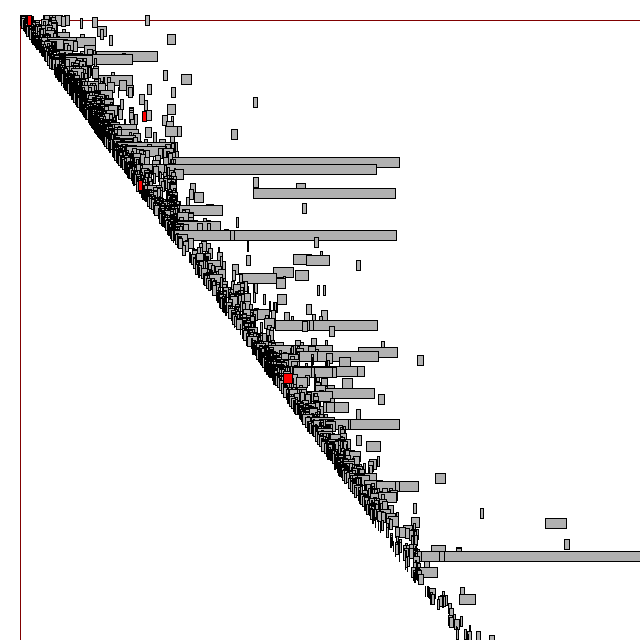
\includegraphics[width=0.45\linewidth]{figures/top_requested.png}
  \label{fig:top_req}
}
\subfloat[Accepted]{
  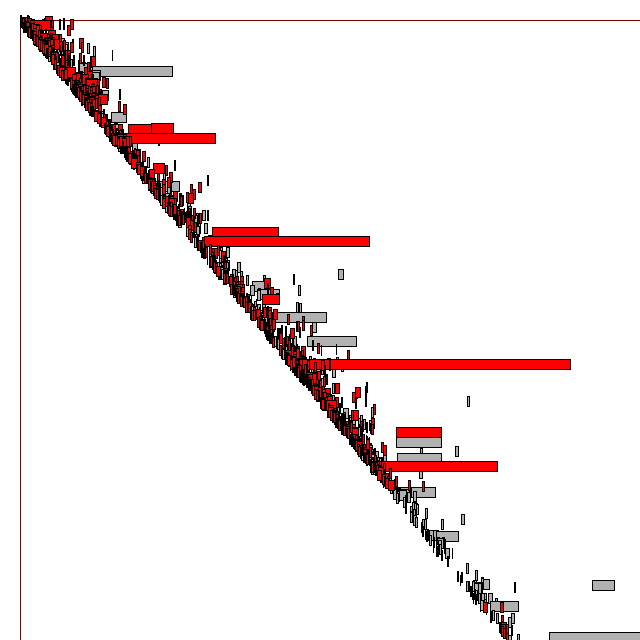
\includegraphics[width=0.45\linewidth]{figures/top_accepted.png}
  \label{fig:top_acc}
}
\caption{Couchrequest for two extreme users}
\label{fig:timeline_view}
\end{figure}
